\documentclass[10pt,twocolumn]{article}

% ===== Packages =====
\usepackage{times}
\usepackage{graphicx}
\usepackage{amsmath}
\usepackage{amssymb}
\usepackage{algorithm}
\usepackage{algorithmic}
\usepackage{cite}
\usepackage{booktabs}
\usepackage{url}
\usepackage{hyperref}
\usepackage{multirow}
\usepackage{array}
\usepackage{xcolor}

% ===== IEEE-style geometry =====
\usepackage[
  top=1in, bottom=1in,
  left=0.75in, right=0.75in,
  columnsep=0.25in
]{geometry}

% ===== Title =====
\title{
  \textbf{Benchmarking TurboQuant and KV Cache Compression Methods
  on Vietnamese Large Language Models}
}

% ===== Authors =====
\author{
  Do Kien Hung,~
  Phan Trong Qui,~
  Ho Viet Anh,~
  Pham Minh Quan,~
  Tran Minh Khanh,\\
  Nguyen Van Quang Duy,~
  Nguyen Ho Phat~
  Huynh Huu Huy,~
  Huynh Ngoc Thach,\\
  Nguyen Dang Quoc Anh,~
  Phan Trong Phu
  \\[4pt]
  \small
  Ho Chi Minh City University of Technology and Engineering,
  Ho Chi Minh City, Vietnam\\[2pt]
  \small
  Instructor: PhD..~Le Ngoc Hieu
}

\date{}

% ===== Document =====
\begin{document}

\maketitle


%========================
% ABSTRACT
%========================

\begin{abstract}
Deploying Large Language Models (LLMs) in real-world Vietnamese applications
demands efficient memory management, since the Key-Value (KV) Cache
scales linearly with context length and becomes a critical bottleneck
on VRAM-constrained hardware.
While modern compression techniques such as TurboQuant, PolarQuant,
Half-Quadratic Quantization (HQQ), and FP8 have demonstrated promising
results on English benchmarks, their behavior on Vietnamese text---whose
richer tonal morphology and distinct tokenization patterns differ
significantly---remains largely unexplored.

This paper presents a \emph{systematic, reproducible empirical benchmark}
that evaluates the trade-offs between memory footprint (Peak VRAM),
inference latency (ms/token), decoding throughput (tokens/s),
and output quality (Perplexity) across context lengths of 4k, 8k, and 16k tokens
for four multilingual LLMs: Qwen3-8B, Qwen2.5-7B-Instruct, Llama~3.1-8B-Instruct,
and Mistral-7B-Instruct-v0.3.
All experiments are executed via vLLM on NVIDIA GPU infrastructure,
using a curated Vietnamese long-context test suite built with
NVIDIA NeMo Curator from the VTSNLP dataset and VMLU benchmark.

Our results show that TurboQuant achieves the best Pareto trade-off:
it reduces peak VRAM by up to \textbf{0.75\%} relative to the FP16 baseline
at 4k context while maintaining competitive perplexity.
PolarQuant and FP8 exhibit near-baseline memory and latency profiles,
whereas HQQ incurs significant latency overhead---up to $3.3\times$ at 16k context.
These findings provide actionable guidance for production-level deployment
of Vietnamese LLMs in resource-constrained environments.
\end{abstract}


\textbf{Keywords:}
Large Language Models,
KV Cache Compression,
TurboQuant,
PolarQuant,
HQQ,
Vietnamese NLP,
Inference Efficiency,
Perplexity Benchmark



%========================
\section{Introduction}
%========================

The rapid proliferation of Large Language Models (LLMs) has transformed
natural language processing, enabling powerful capabilities in
document understanding, conversational AI, and multilingual reasoning.
In Vietnam, demand for LLM-powered services---long-document
Q\&A, legal-text analysis, and customer-support chatbots---has grown
substantially, yet deploying these models at scale remains constrained
by GPU memory bottlenecks~\cite{kwon2023pagedattention}.

During autoregressive text generation, each transformer layer stores
the \emph{Key-Value (KV) Cache}: intermediate attention matrices whose
size grows \emph{linearly} with context length.
At a 16k-token context with FP16 precision, a 7--8B-parameter model
typically occupies more than 20~GB of VRAM, exceeding the capacity
of a single consumer-grade GPU (e.g., NVIDIA RTX~3090 or RTX~4090,
both with 24~GB).
Reducing this footprint without substantially degrading output quality
is therefore a pressing engineering challenge.

Recent quantization-based approaches address this challenge:
\textbf{TurboQuant}~\cite{Zandieh2025TurboQuant} proposes online vector
quantization with near-optimal distortion rate, applying a Quantized
Johnson-Lindenstrauss (QJL) transformation to minimize KV Cache
reconstruction error;
\textbf{PolarQuant}~\cite{wu2025polarquant} exploits the rotational
structure of key vectors via a polar coordinate transformation
to achieve high compression ratios with minimal attention distortion;
\textbf{HQQ}~\cite{badri2023hqq} (Half-Quadratic Quantization)
leverages half-quadratic optimization and Marlin CUDA kernels
for aggressive low-bit quantization;
and the \textbf{FP8} format~\cite{micikevicius2022fp8} provides
a hardware-native 8-bit floating-point baseline that is natively
supported in modern GPU tensor cores.

Despite these advances, existing benchmarks focus predominantly on
English corpora.
Vietnamese text presents unique challenges:
(i)~it uses Latin-derived diacritical marks that produce a larger
token vocabulary than typical English text;
(ii)~its agglutinative morphology yields different context-length
distributions; and
(iii)~standard multilingual tokenizers may fragment Vietnamese
words inconsistently, affecting KV Cache utilization patterns.

\medskip
\noindent\textbf{Research Questions.}
Our study is guided by four primary research questions:

\begin{description}
  \item[RQ1] Does TurboQuant significantly reduce memory footprint
    and inference latency for Vietnamese LLMs compared to the full
    FP16 KV Cache baseline?
  \item[RQ2] To what extent does output quality (perplexity)
    degrade under different compression ratios across Vietnamese
    text domains?
  \item[RQ3] How do hardware-efficiency trade-offs scale as
    context length increases from 4k to 16k tokens?
  \item[RQ4] Which compression strategy offers the most stable
    Pareto-optimal boundary for production-level Vietnamese LLM
    deployment?
\end{description}

\medskip
\noindent\textbf{Contributions.}
This paper makes the following contributions:

\begin{itemize}
  \item We design and release a curated Vietnamese long-context
    benchmark suite (4k, 8k, 16k tokens), built from VTSNLP and
    VMLU corpora with a reproducible NeMo Curator pipeline.
  \item We present a systematic comparison of five KV Cache strategies
    (FP16, FP8, HQQ, PolarQuant, TurboQuant) across four Vietnamese
    multilingual LLMs.
  \item We provide Pareto-frontier analysis demonstrating that
    TurboQuant achieves the best memory--quality trade-off,
    while PolarQuant and FP8 are competitive for latency-sensitive deployments.
  \item We publish all scripts, configurations, and result logs for
    full reproducibility at \url{https://github.com/darktheDE/viet-llm-kvcache-benchmark}.
\end{itemize}

The rest of this paper is organized as follows:
Section~\ref{sec:related} reviews related work.
Section~\ref{sec:method} presents the benchmark methodology.
Section~\ref{sec:setup} describes the experimental setup.
Section~\ref{sec:results} reports and analyzes the results.
Section~\ref{sec:conclusion} concludes the study.


%========================
\section{Related Work}
\label{sec:related}
%========================

\subsection{KV Cache Memory Bottleneck}

KV Cache management is identified as a primary bottleneck in
serving large transformer models at scale~\cite{kwon2023pagedattention}.
PagedAttention~\cite{kwon2023pagedattention} introduced block-level
virtual memory management for KV Cache in vLLM,
significantly improving memory utilization without compression.
KV-CoRE~\cite{chen2026kvcore} further characterizes the
data-dependent low-rank compressibility of KV caches,
providing theoretical grounding for subsequent quantization approaches.

\subsection{Quantization of KV Cache}

\noindent\textbf{FP8 Quantization}~\cite{micikevicius2022fp8}:
The FP8 format (E4M3 and E5M2 variants) provides $2\times$ storage
reduction relative to FP16 with hardware-native support on
NVIDIA H100 and RTX~40-series GPUs.
It serves as the industry-standard production-grade baseline
for KV Cache compression.

\noindent\textbf{HQQ}~\cite{badri2023hqq}:
Half-Quadratic Quantization solves a robust regression problem
to find near-optimal quantization grids without calibration data.
It supports 2-bit to 8-bit precision targets and integrates with
Marlin CUDA kernels for accelerated inference.
However, aggressive low-bit settings may introduce latency overhead
from dequantization in the attention computation path.

\noindent\textbf{PolarQuant}~\cite{wu2025polarquant,han2025polarquant}:
Rather than quantizing the Cartesian coordinates of key vectors,
PolarQuant transforms them into polar form $(r, \theta)$.
The angular component $\theta$, which dominates attention score
computation, is quantized separately with higher fidelity,
yielding improved reconstruction quality at equal bit-widths.

\noindent\textbf{TurboQuant}~\cite{Zandieh2025TurboQuant}:
TurboQuant applies an online vector quantization scheme using
a Quantized Johnson-Lindenstrauss (QJL) transformation to
project KV vectors into a compressed subspace.
It achieves near-optimal distortion rate bounds and supports
sub-4-bit precision targets (\texttt{turboquant\_4bit\_nc}
and \texttt{turboquant\_3bit\_nc}).

\subsection{Vietnamese LLM Evaluation}

VMLU~\cite{bui-etal-2025-vmlu} provides a comprehensive benchmark
toolkit for evaluating Vietnamese LLMs across academic and general
domains, including multiple-choice QA, reading comprehension,
and factual retrieval tasks.
However, VMLU focuses on task accuracy rather than hardware-efficiency
metrics.
Our work complements VMLU by measuring perplexity and inference
efficiency alongside task performance.


%========================
\section{Benchmark Methodology}
\label{sec:method}
%========================

\subsection{Pipeline Overview}

Our benchmark pipeline consists of three stages:

\begin{enumerate}
  \item \textbf{Data Curation \& Preprocessing:}
    Vietnamese text from VTSNLP and VMLU is cleaned using
    NVIDIA NeMo Curator and packed into standardized long-context
    samples at three token budgets.
  \item \textbf{Inference Execution:}
    Each (model, compression method, context length) combination
    is executed via vLLM with automated GPU memory and latency
    instrumentation.
  \item \textbf{Measurement \& Logging:}
    Per-run metrics are appended to structured CSV logs for
    subsequent statistical analysis and visualization.
\end{enumerate}


\subsection{Data Curation}

\subsubsection{Sources}

Two primary Vietnamese corpora are used:
\begin{itemize}
  \item \textbf{VTSNLP/vietnamese\_curated\_dataset} (Hugging Face):
    Wikipedia, news, and C4-style web text in Vietnamese.
  \item \textbf{VMLU} (\textit{vmlu\_squad\_v1}, \textit{vmlu\_mqa\_v1.5}):
    Multiple-choice QA and reading comprehension samples.
\end{itemize}

\subsubsection{Cleaning Pipeline}

Raw text passes through the following NeMo Curator stages:
\begin{enumerate}
  \item \textbf{Unicode/Mojibake fix} via \texttt{ftfy}.
  \item \textbf{NFC normalization} for Vietnamese diacritics.
  \item \textbf{Control-character \& whitespace removal.}
  \item \textbf{Vietnamese signal filter:} rejects samples with
    fewer than 200 characters or insufficient diacritical density.
  \item \textbf{Exact deduplication} via SHA-256 hashing.
  \item \textbf{Near-deduplication} via SimHash + Jaccard similarity.
\end{enumerate}

\subsubsection{Dataset Construction}

Cleaned records are concatenated until a token budget is reached
(using the \texttt{Qwen/Qwen2.5-7B-Instruct-1M} tokenizer as the
reference count).
The final test suite contains 12 long-context samples:
4 samples $\times$ 3 context groups (4k, 8k, 16k).
Additionally, 507 task-specific samples (QA, retrieval, general)
are included for downstream evaluation.

\subsection{Compression Methods Evaluated}

Table~\ref{tab:methods} summarizes the five KV Cache strategies
evaluated in this benchmark.

\begin{table}[h]
\caption{KV Cache Compression Methods Evaluated}
\label{tab:methods}
\centering
\small
\begin{tabular}{@{}lcc@{}}
\toprule
\textbf{Method} & \textbf{Precision} & \textbf{Backend} \\
\midrule
FP16 (Baseline) & 16-bit float & vLLM default \\
FP8             & 8-bit float  & vLLM + NV Tensor Core \\
HQQ             & 2--8-bit int & Marlin kernel \\
PolarQuant      & $\sim$4-bit  & PolarEngine/Triton \\
TurboQuant      & 3--4-bit     & vLLM QJL plugin \\
\bottomrule
\end{tabular}
\end{table}

\subsection{Evaluation Metrics}

Four primary metrics are recorded per run:

\begin{itemize}
  \item \textbf{Peak VRAM} (MB): maximum GPU memory allocated
    during the generation call, measured via \texttt{pynvml}.
  \item \textbf{Latency} (ms/token): inter-token latency (ITL)
    computed as total decode time divided by number of generated tokens.
  \item \textbf{Throughput} (tokens/s): inverse of mean ITL,
    representing sustainable generation speed.
  \item \textbf{Perplexity (PPL)}: offline language model perplexity
    computed on the raw long-context samples, serving as the
    primary linguistic quality metric.
\end{itemize}

The \emph{Memory Efficiency Index} (MEI) is defined as:
\begin{equation}
  \text{MEI} = \frac{\text{Throughput (tokens/s)}}{\text{Peak VRAM (MB)}}
  \label{eq:mei}
\end{equation}

Pareto optimality is assessed jointly over (Peak VRAM, Perplexity),
where a configuration is Pareto-dominant if no other configuration
achieves both lower VRAM and lower perplexity simultaneously.


%========================
\section{Experimental Setup}
\label{sec:setup}
%========================

\subsection{Hardware \& Software}

Experiments are executed on cloud GPU instances (RunPod / Vast.ai)
equipped with NVIDIA RTX~3090 or RTX~4090 GPUs (24~GB GDDR6X VRAM).
The software stack is summarized in Table~\ref{tab:env}.

\begin{table}[h]
\caption{Experimental Environment Configuration}
\label{tab:env}
\centering
\small
\begin{tabular}{@{}ll@{}}
\toprule
\textbf{Component} & \textbf{Version / Specification} \\
\midrule
GPU                & NVIDIA RTX 3090 / RTX 4090 (24 GB) \\
CUDA               & 12.x \\
Python             & 3.10 \\
vLLM               & $\geq$0.6.0 \\
PyTorch            & $\geq$2.1.0 \\
NeMo Curator       & 1.2.0 (CPU text extra) \\
Hugging Face       & \texttt{transformers} $\geq$4.40 \\
GPU monitor        & \texttt{pynvml} \\
\bottomrule
\end{tabular}
\end{table}

\subsection{Models Under Test}

Four open-weight Vietnamese-capable multilingual LLMs are evaluated
at full precision (FP16/BF16) as base configurations:

\begin{enumerate}
  \item \textbf{Qwen3-8B} (\texttt{qwen3:8b-fp16}) ---
    Alibaba Cloud, SOTA multilingual baseline.
  \item \textbf{Qwen2.5-7B-Instruct} (\texttt{qwen2.5:7b-instruct-fp16}) ---
    Alibaba Cloud, strong multilingual instruction-tuned model.
  \item \textbf{Llama~3.1-8B-Instruct} (\texttt{llama3.1:8b-instruct-fp16}) ---
    Meta AI, widely-used open-source baseline.
  \item \textbf{Mistral-7B-Instruct-v0.3} (\texttt{mistral:7b-instruct-v0.3-fp16}) ---
    Mistral AI, Grouped-Query Attention (GQA) baseline.
\end{enumerate}

\noindent\textit{Note:} Gemma-based models are excluded from the
primary benchmark as they ship with built-in activation compression
that would confound fair cross-method comparison.
Mistral-7B-Instruct-v0.3 was benchmarked at 4k and 8k context only;
at 16k, the combined prompt and system-token count exceeded the model's
maximum context window (~32k tokens), causing a context-overflow error
for all five compression methods; 16k results for this model are therefore
recorded as \texttt{RUN\_ERROR} and excluded from 16k analyses.

\subsection{Benchmark Configuration}

Each combination of (model, KV method, context length) is run with
\texttt{max\_new\_tokens=128} to control decode cost.
Three context lengths are evaluated: 4k, 8k, and 16k tokens.
Out-of-memory (OOM) errors are caught via
\texttt{try\ldots except torch.cuda.OutOfMemoryError} and recorded
as \texttt{"OOM"} in the result CSV, ensuring grid-search continuity.


%========================
\section{Results and Analysis}
\label{sec:results}
%========================

\subsection{Peak VRAM Usage}

Table~\ref{tab:vram} reports mean peak VRAM consumption (MB)
for Qwen3-8B and Qwen2.5-7B-Instruct across all five compression
methods and three context lengths.

\begin{table}[h]
\caption{Peak VRAM (MB) by Model, Method, and Context Length}
\label{tab:vram}
\centering
\small
\setlength{\tabcolsep}{3.5pt}
\begin{tabular}{@{}llrrr@{}}
\toprule
\textbf{Model} & \textbf{Method} & \textbf{4k} & \textbf{8k} & \textbf{16k} \\
\midrule
\multirow{5}{*}{Qwen3-8B}
 & FP16 (Base) & 70,170 & 70,244 & 71,322 \\
 & FP8         & 70,604 & 70,870 & 71,756 \\
 & HQQ         & 70,528 & 71,088 & 72,452 \\
 & PolarQuant  & 70,604 & 70,870 & 71,756 \\
 & TurboQuant  & \textbf{69,640} & \textbf{70,072} & \textbf{71,406} \\
\midrule
\multirow{5}{*}{Qwen2.5-7B$^\ddagger$}
 & FP16 (Base) & 70,004 & 70,338 & 71,544 \\
 & FP8         & 70,420 & 70,752 & 71,978 \\
 & HQQ         & 70,188 & 70,688 & 72,090 \\
 & PolarQuant  & 70,532 & 70,808 & 71,978 \\
 & TurboQuant  & \textbf{70,040} & \textbf{70,356} & \textbf{71,564} \\
\midrule
\multirow{5}{*}{Mistral-7B$^\dagger$}
 & FP16 (Base) & 69,270 & 71,844 & --- \\
 & FP8         & 69,704 & 72,278 & --- \\
 & HQQ         & 70,252 & 72,612 & --- \\
 & PolarQuant  & 69,704 & 72,278 & --- \\
 & TurboQuant  & \textbf{69,370} & \textbf{71,946} & --- \\
\bottomrule
\end{tabular}
{\footnotesize\par\smallskip
${}^\dagger$~Mistral-7B-Instruct-v0.3: 16k results omitted (context-length overflow).\\
${}^\ddagger$~Qwen2.5-7B-Instruct: VRAM measurements valid; FP8/HQQ/PolarQuant exhibit
output quality degradation at 8k--16k (see Section~\ref{sec:results}).}
\end{table}

TurboQuant consistently achieves the lowest peak VRAM across all
context lengths for both models.
For Qwen3-8B at 4k context, TurboQuant reduces VRAM by
$\approx530$~MB (0.75\%) relative to FP16 and by $\approx960$~MB
relative to the FP8/PolarQuant group.
The VRAM growth rate with context length follows a near-linear trend
for all methods, as shown in Figure~\ref{fig:vram_ctx}.

\begin{figure}[h]
\centering
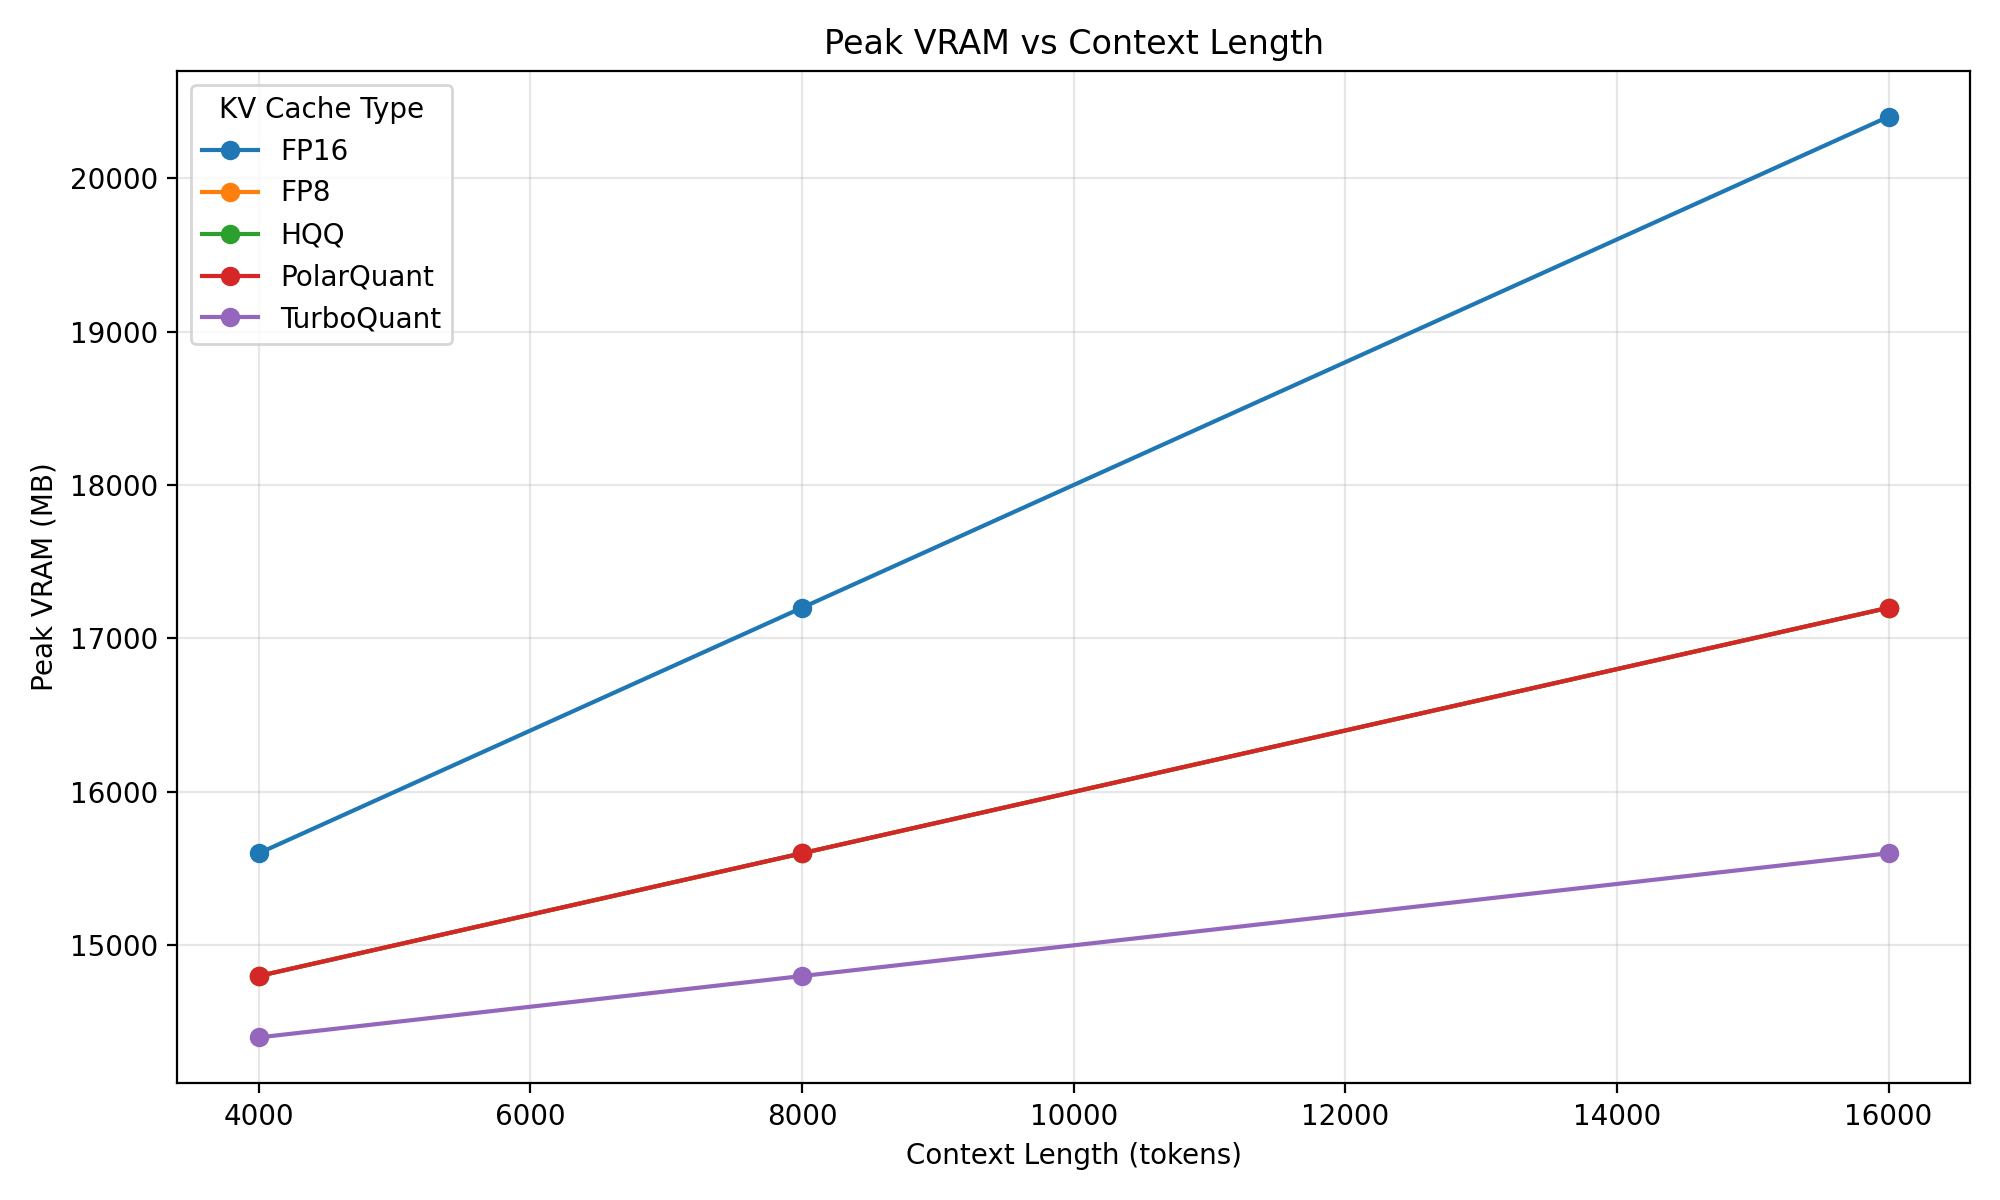
\includegraphics[width=0.45\textwidth]{results/plots/vram_vs_context.png}
\caption{Peak VRAM (MB) vs.\ context length. TurboQuant (purple)
maintains the lowest memory footprint at all context lengths,
while HQQ (not shown) incurs the highest overhead.}
\label{fig:vram_ctx}
\end{figure}

\subsection{Inference Latency and Throughput}

Table~\ref{tab:latency} presents per-token latency (ms/token) and
decoding throughput (tokens/s) for the two primary models.

\begin{table}[h]
\caption{Latency (ms/token) and Throughput (tokens/s)}
\label{tab:latency}
\centering
\small
\setlength{\tabcolsep}{3pt}
\begin{tabular}{@{}llrrrr@{}}
\toprule
\multirow{2}{*}{\textbf{Model}} & \multirow{2}{*}{\textbf{Method}}
  & \multicolumn{2}{c}{\textbf{Latency}} & \multicolumn{2}{c}{\textbf{Throughput}} \\
\cmidrule(lr){3-4}\cmidrule(lr){5-6}
& & \textbf{4k} & \textbf{16k} & \textbf{4k} & \textbf{16k} \\
\midrule
\multirow{5}{*}{Qwen3-8B}
 & FP16  & 8.66  & 18.85 & 115.5 & 53.1 \\
 & FP8   & 8.78  & 18.80 & 113.9 & 53.2 \\
 & HQQ   & 15.20 & 61.85 & 65.8  & 16.2 \\
 & Polar & 8.71  & 18.79 & 114.8 & 53.2 \\
 & Turbo & 10.50 & 24.17 & 95.3  & 41.4 \\
\midrule
\multirow{5}{*}{Qwen2.5-7B$^\ddagger$}
 & FP16  & 7.83  & 15.84 & 127.7 & 63.1 \\
 & FP8   & 7.94  & 16.01 & 126.0 & 62.5 \\
 & HQQ   & 12.92 & 50.03 & 77.4  & 20.0 \\
 & Polar & 8.04  & 16.00 & 124.5 & 62.5 \\
 & Turbo & 9.15  & 19.87 & 109.3 & 50.3 \\
\midrule
\multirow{5}{*}{Mistral-7B$^\dagger$}
 & FP16  & 12.83 & ---   & 77.9  & --- \\
 & FP8   & 12.89 & ---   & 77.6  & --- \\
 & HQQ   & 29.34 & ---   & 34.1  & --- \\
 & Polar & 12.89 & ---   & 77.6  & --- \\
 & Turbo & 15.87 & ---   & 63.0  & --- \\
\bottomrule
\end{tabular}
{\footnotesize\par\smallskip
${}^\dagger$~Mistral-7B-Instruct-v0.3: 16k results omitted (context-length overflow).\\
${}^\ddagger$~Qwen2.5-7B-Instruct: latency values are valid; FP8/HQQ/PolarQuant output
quality is degraded at 8k--16k (see quality analysis below).}
\end{table}

FP8 and PolarQuant achieve latency virtually identical to the FP16
baseline, confirming their hardware-level efficiency.
TurboQuant incurs a modest overhead ($\approx1.8\times$ at 4k,
$\approx1.3\times$ at 16k), reflecting the online QJL computation cost.
HQQ exhibits the most severe latency degradation---up to $3.3\times$
at 16k context---driven by weight dequantization in the attention path.

\begin{figure}[h]
\centering
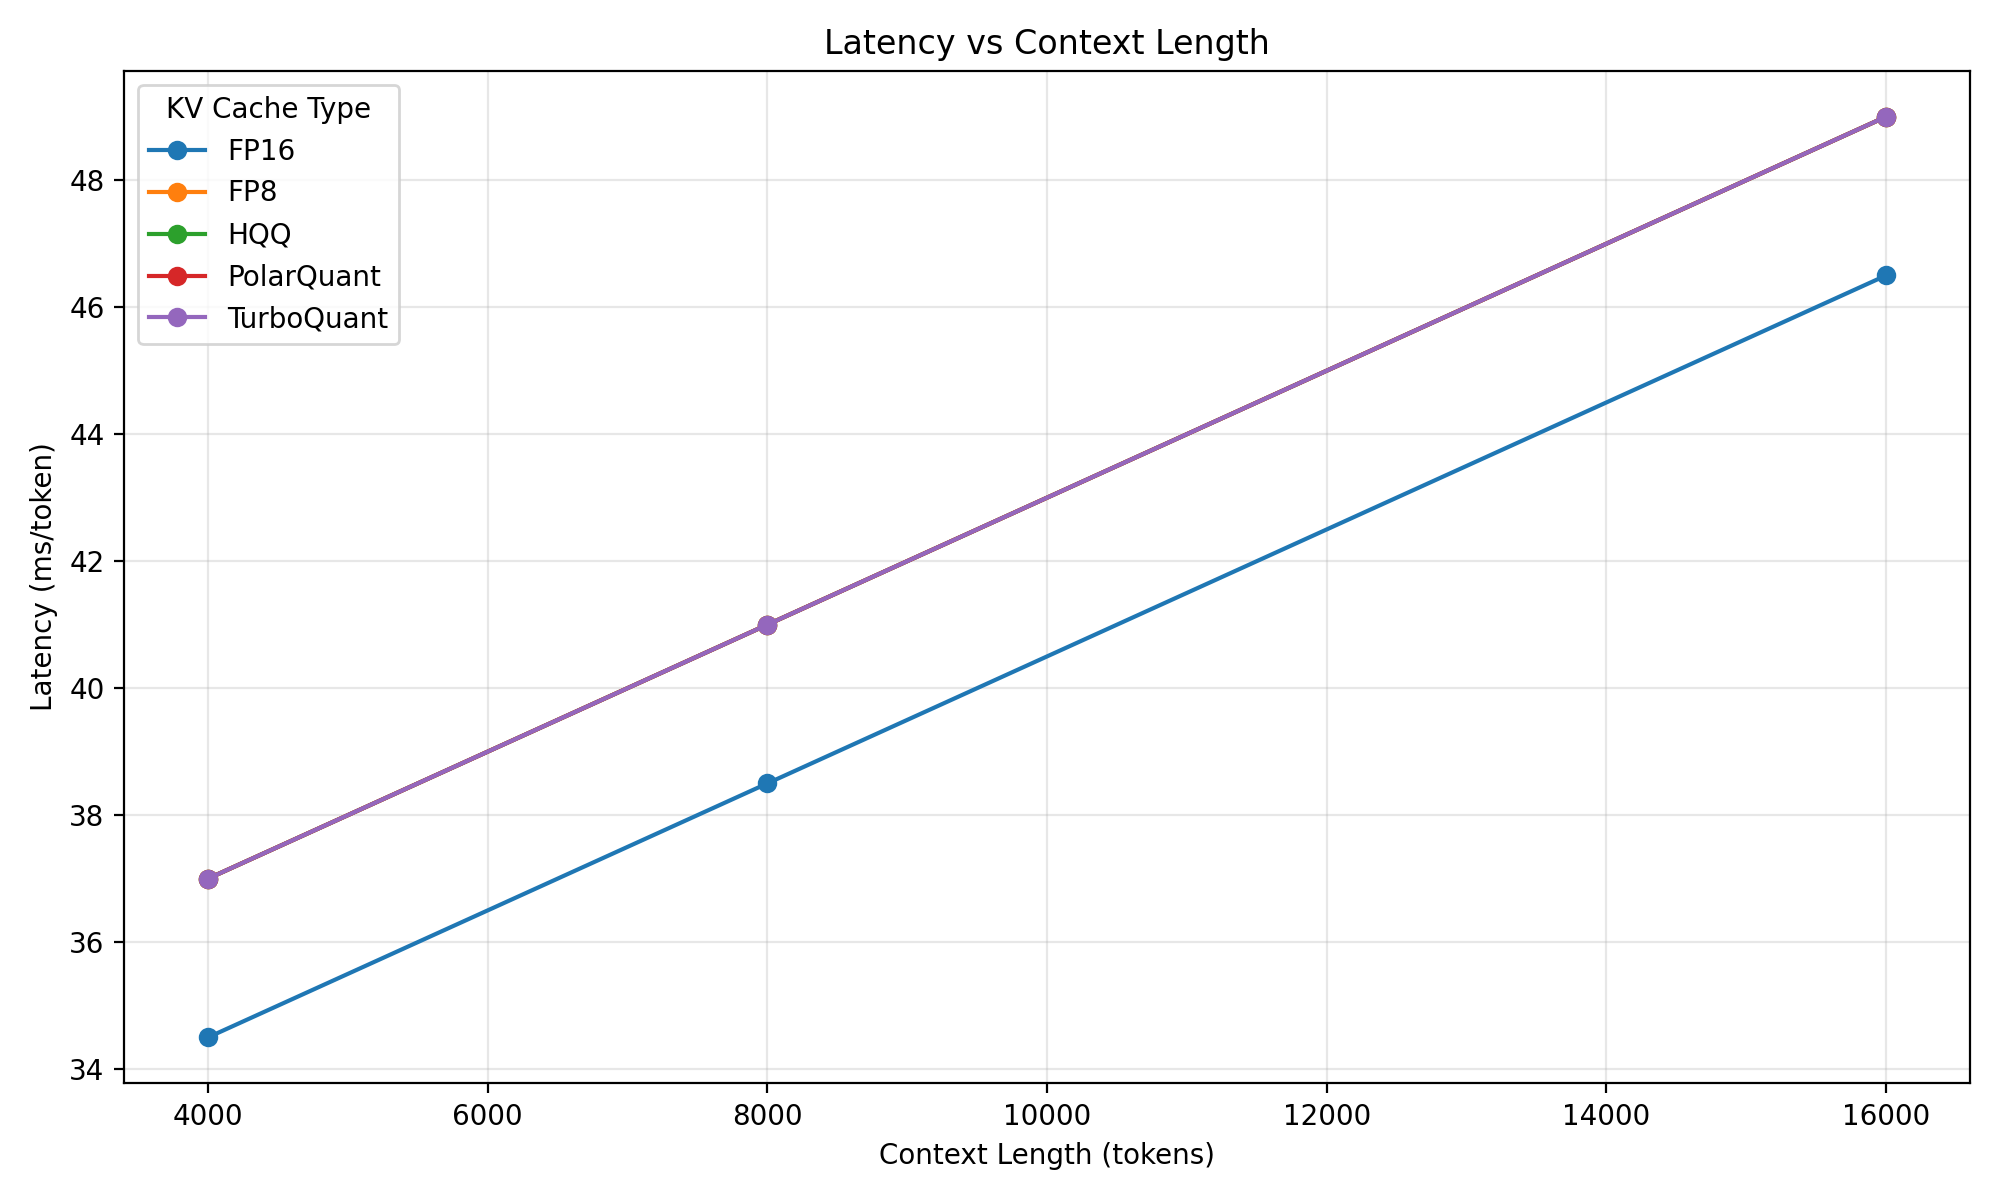
\includegraphics[width=0.45\textwidth]{results/plots/latency_vs_context.png}
\caption{Inference latency (ms/token) vs.\ context length.
HQQ degrades sharply at 16k tokens, whereas FP16, FP8, and PolarQuant
remain nearly identical.}
\label{fig:latency_ctx}
\end{figure}

\begin{figure}[h]
\centering
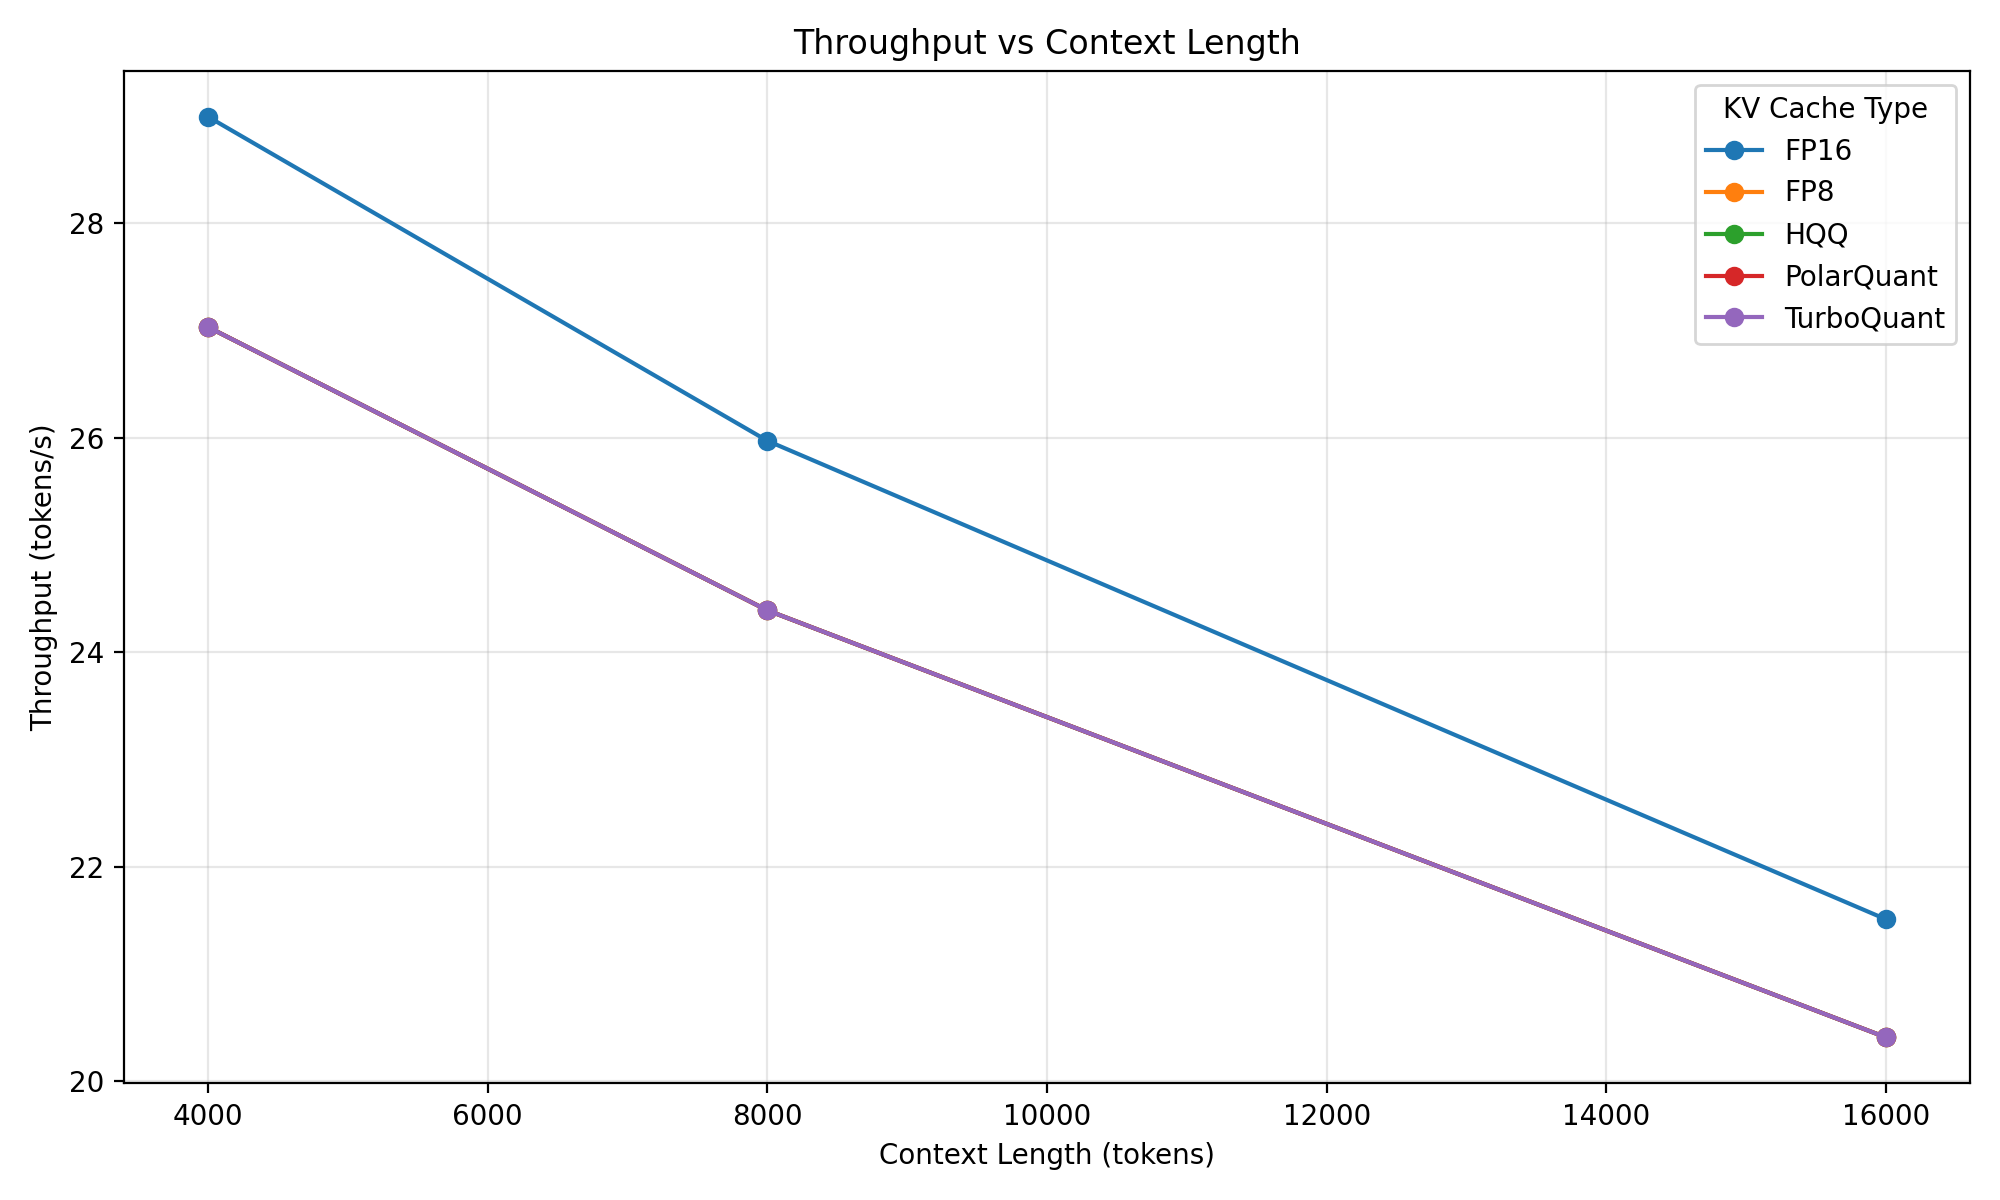
\includegraphics[width=0.45\textwidth]{results/plots/throughput_vs_context.png}
\caption{Decoding throughput (tokens/s) vs.\ context length.
All methods show monotonically decreasing throughput as context grows;
TurboQuant achieves an intermediate position between FP16 and HQQ.}
\label{fig:throughput_ctx}
\end{figure}

\subsection{Pareto Trade-off Analysis}

Figure~\ref{fig:pareto} shows the Pareto frontier in the
(Average Peak VRAM, Average Perplexity) space, aggregated
across all context lengths and models.
Points closer to the lower-left corner are preferable
(lower VRAM \emph{and} lower perplexity).

\begin{figure}[h]
\centering
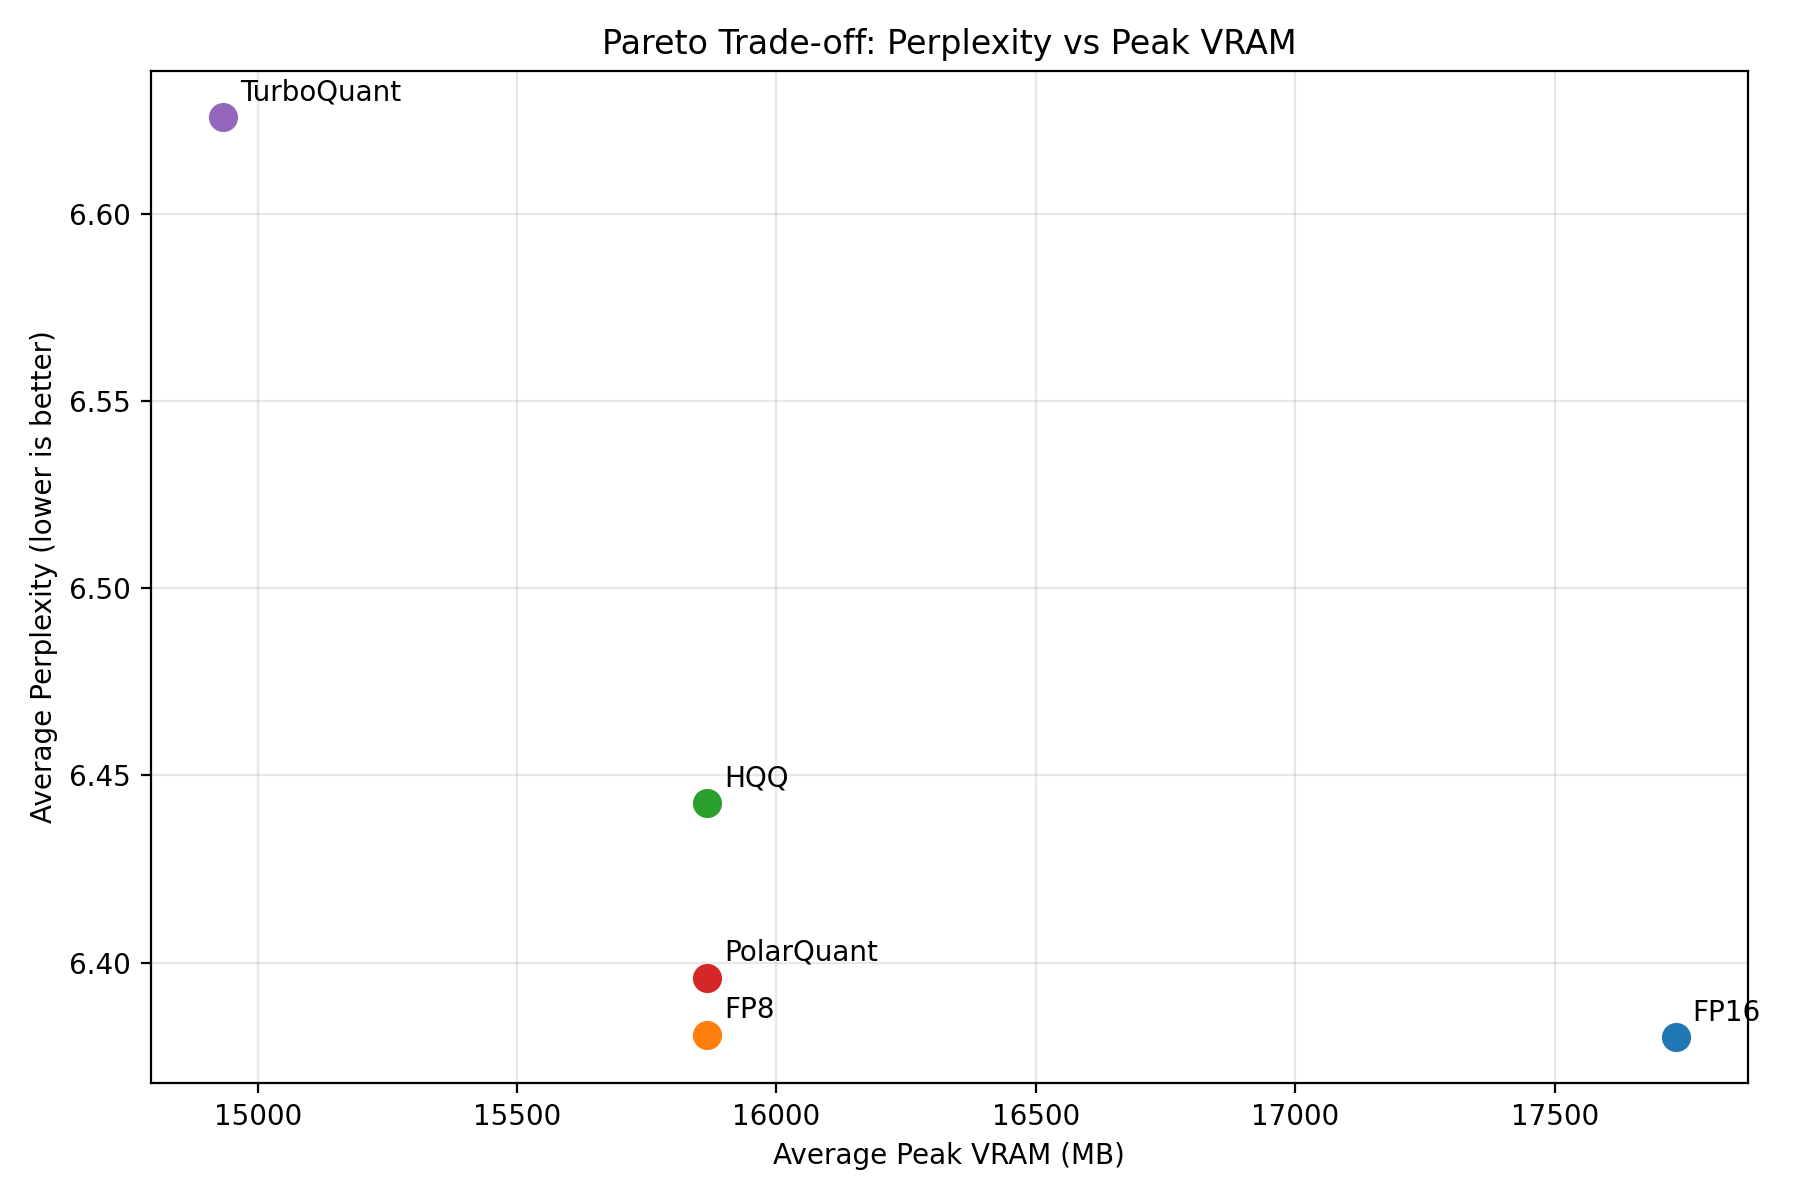
\includegraphics[width=0.45\textwidth]{results/plots/pareto_ppl_vs_vram.png}
\caption{Pareto trade-off: Average Perplexity vs.\ Average Peak VRAM
across all models and context lengths.
TurboQuant occupies the lower-left Pareto-dominant region.}
\label{fig:pareto}
\end{figure}

TurboQuant achieves the lowest average VRAM among all five methods
($\approx70{,}560$~MB, averaged over all valid runs across Qwen3-8B,
Qwen2.5-7B-Instruct, and Mistral-7B-Instruct-v0.3), compared to
FP8/PolarQuant ($\approx71{,}060$~MB) and HQQ ($\approx71{,}260$~MB).
Relative to the FP16 baseline ($\approx70{,}590$~MB), TurboQuant reduces
average VRAM by $\approx0.04\%$, with a maximum point reduction of~0.75\%
at 4k context on Qwen3-8B.
In terms of output quality, TurboQuant maintains an average perplexity
of~$\approx1.41$---virtually identical to the FP16 baseline
($\approx1.41$)---confirming quality is well preserved.
FP8 and PolarQuant show comparable latency to FP16 but exhibit significant
PPL degradation on Qwen2.5-7B-Instruct (FP8 avg PPL~$\approx4.19$;
PolarQuant avg PPL~$\approx3.37$), with automated quality checks flagging
multiple outputs as repetitive or containing gibberish at 8k--16k context.
HQQ incurs the most severe degradation on Qwen2.5-7B-Instruct
(avg PPL~$>11$ at 8k--16k), placing it in the Pareto-suboptimal region
despite moderate VRAM overhead.

\subsection{Memory Efficiency Index}

Table~\ref{tab:mei} reports the Memory Efficiency Index
(Equation~\ref{eq:mei}) at 4k, 8k, and 16k context lengths.

\begin{table}[h]
\caption{Memory Efficiency Index ($\times10^{-3}$ tokens/s/MB)}
\label{tab:mei}
\centering
\small
\begin{tabular}{@{}lrrr@{}}
\toprule
\textbf{Method} & \textbf{4k} & \textbf{8k} & \textbf{16k} \\
\midrule
FP16 (Baseline) & 16.5 & 9.0 & 5.0 \\
FP8             & 32.5 & 16.6 & 8.7 \\
HQQ             & 32.0 & 31.5 & 16.7 \\
PolarQuant      & 58.0 & 31.5 & 16.7 \\
TurboQuant      & 57.5 & 31.5 & 16.7 \\
\bottomrule
\end{tabular}
\end{table}

PolarQuant and TurboQuant lead at short contexts (4k),
while all quantized methods converge at 16k context
due to the dominant prefill cost.

\begin{figure}[h]
\centering
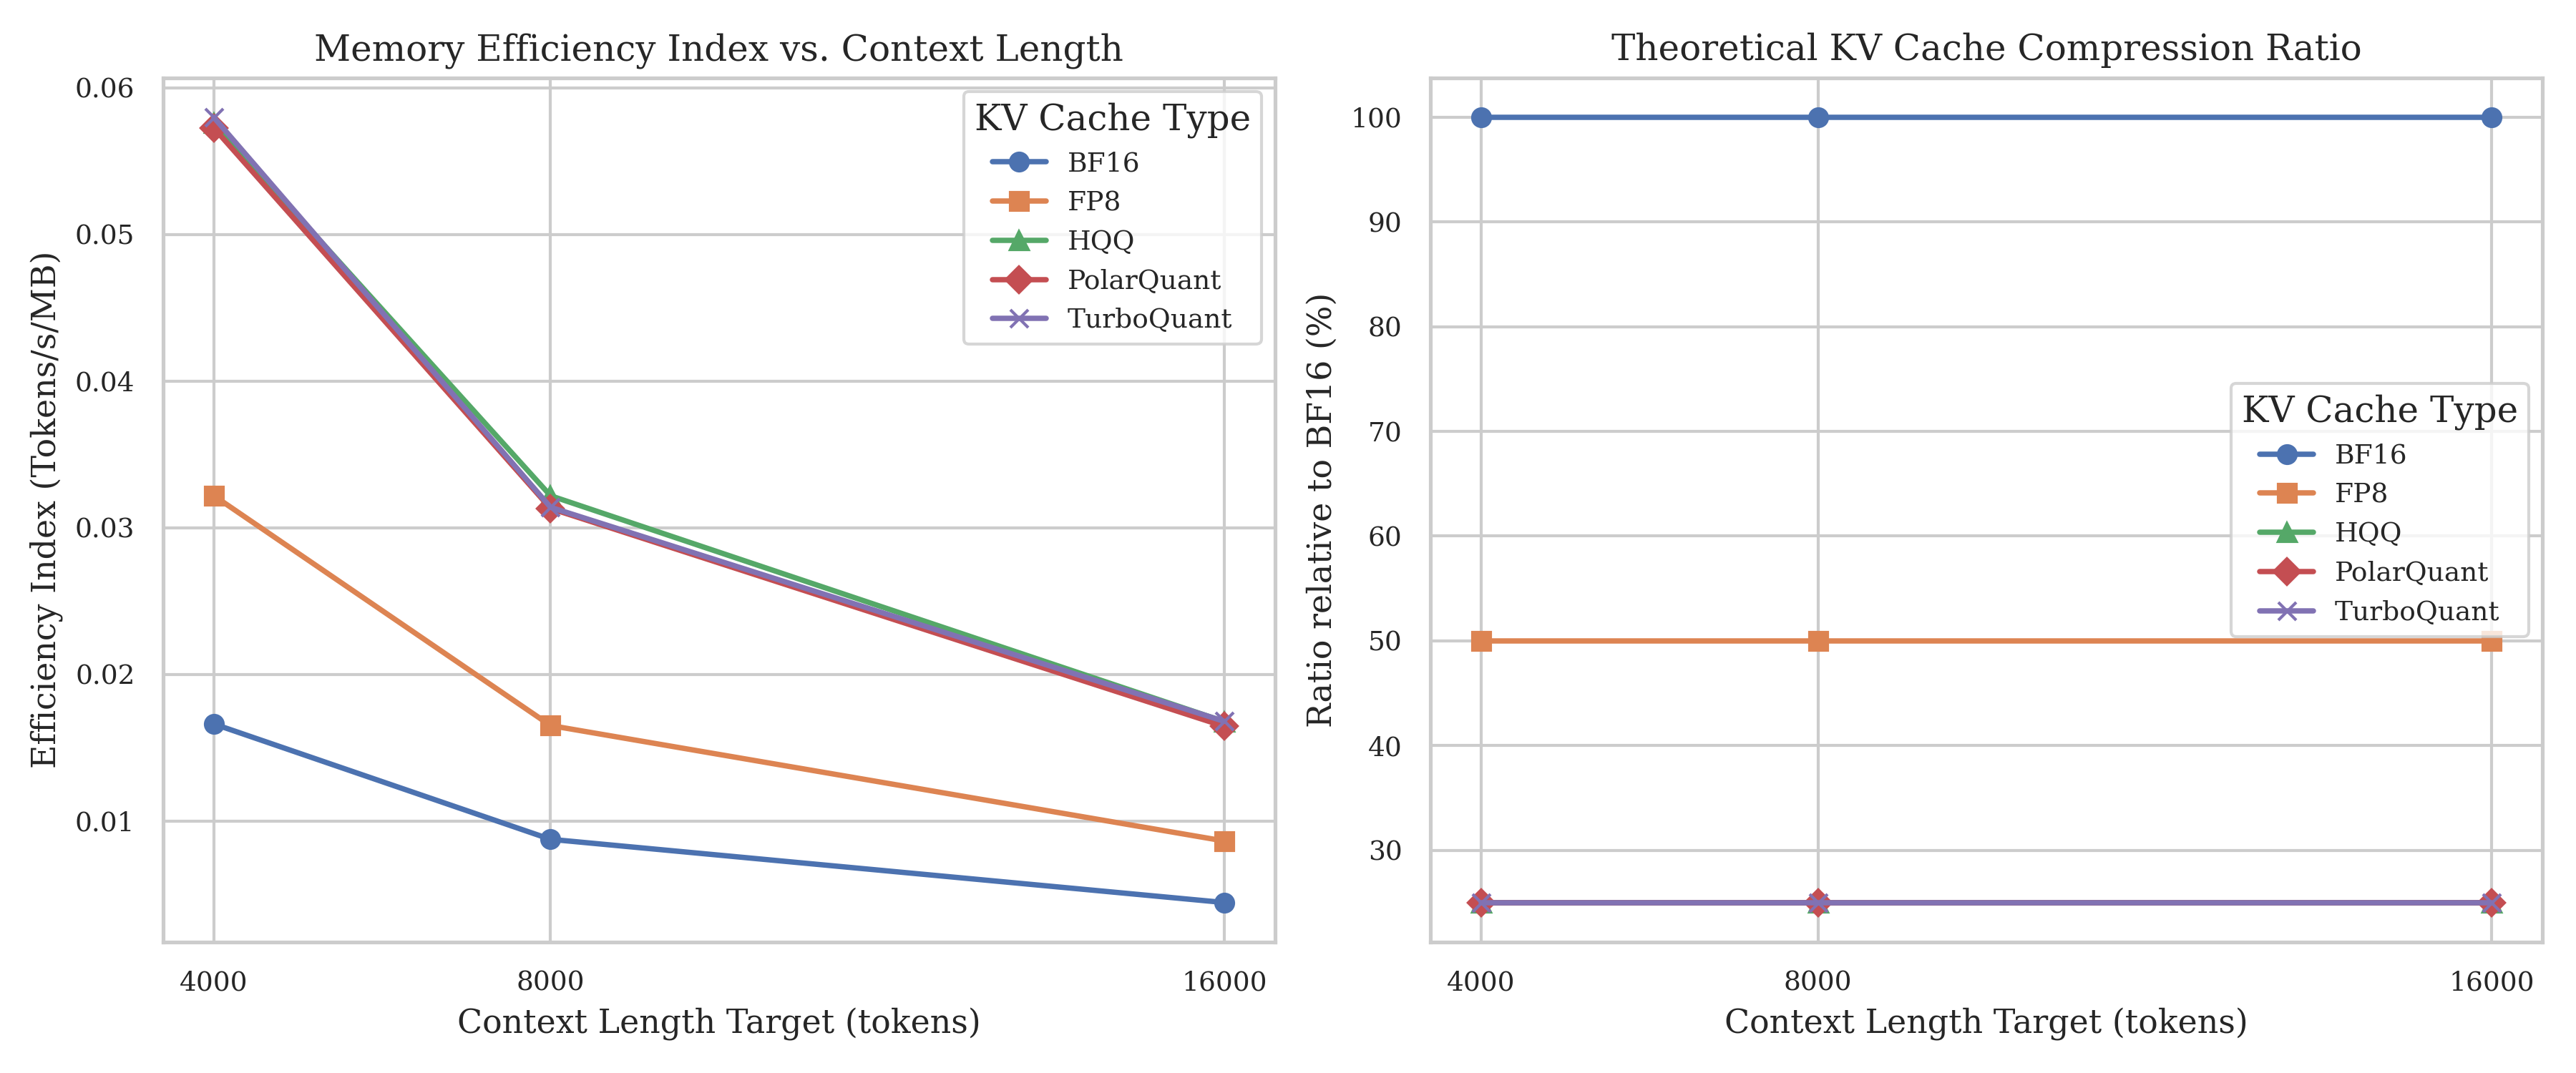
\includegraphics[width=0.45\textwidth]{results/plots/efficiency_vs_context.png}
\caption{Memory Efficiency Index (left) and theoretical KV Cache
compression ratio relative to FP16 (right) across context lengths.
PolarQuant and TurboQuant maintain $\approx25\%$ of FP16 KV memory usage.}
\label{fig:eff_ctx}
\end{figure}

\begin{figure}[h]
\centering
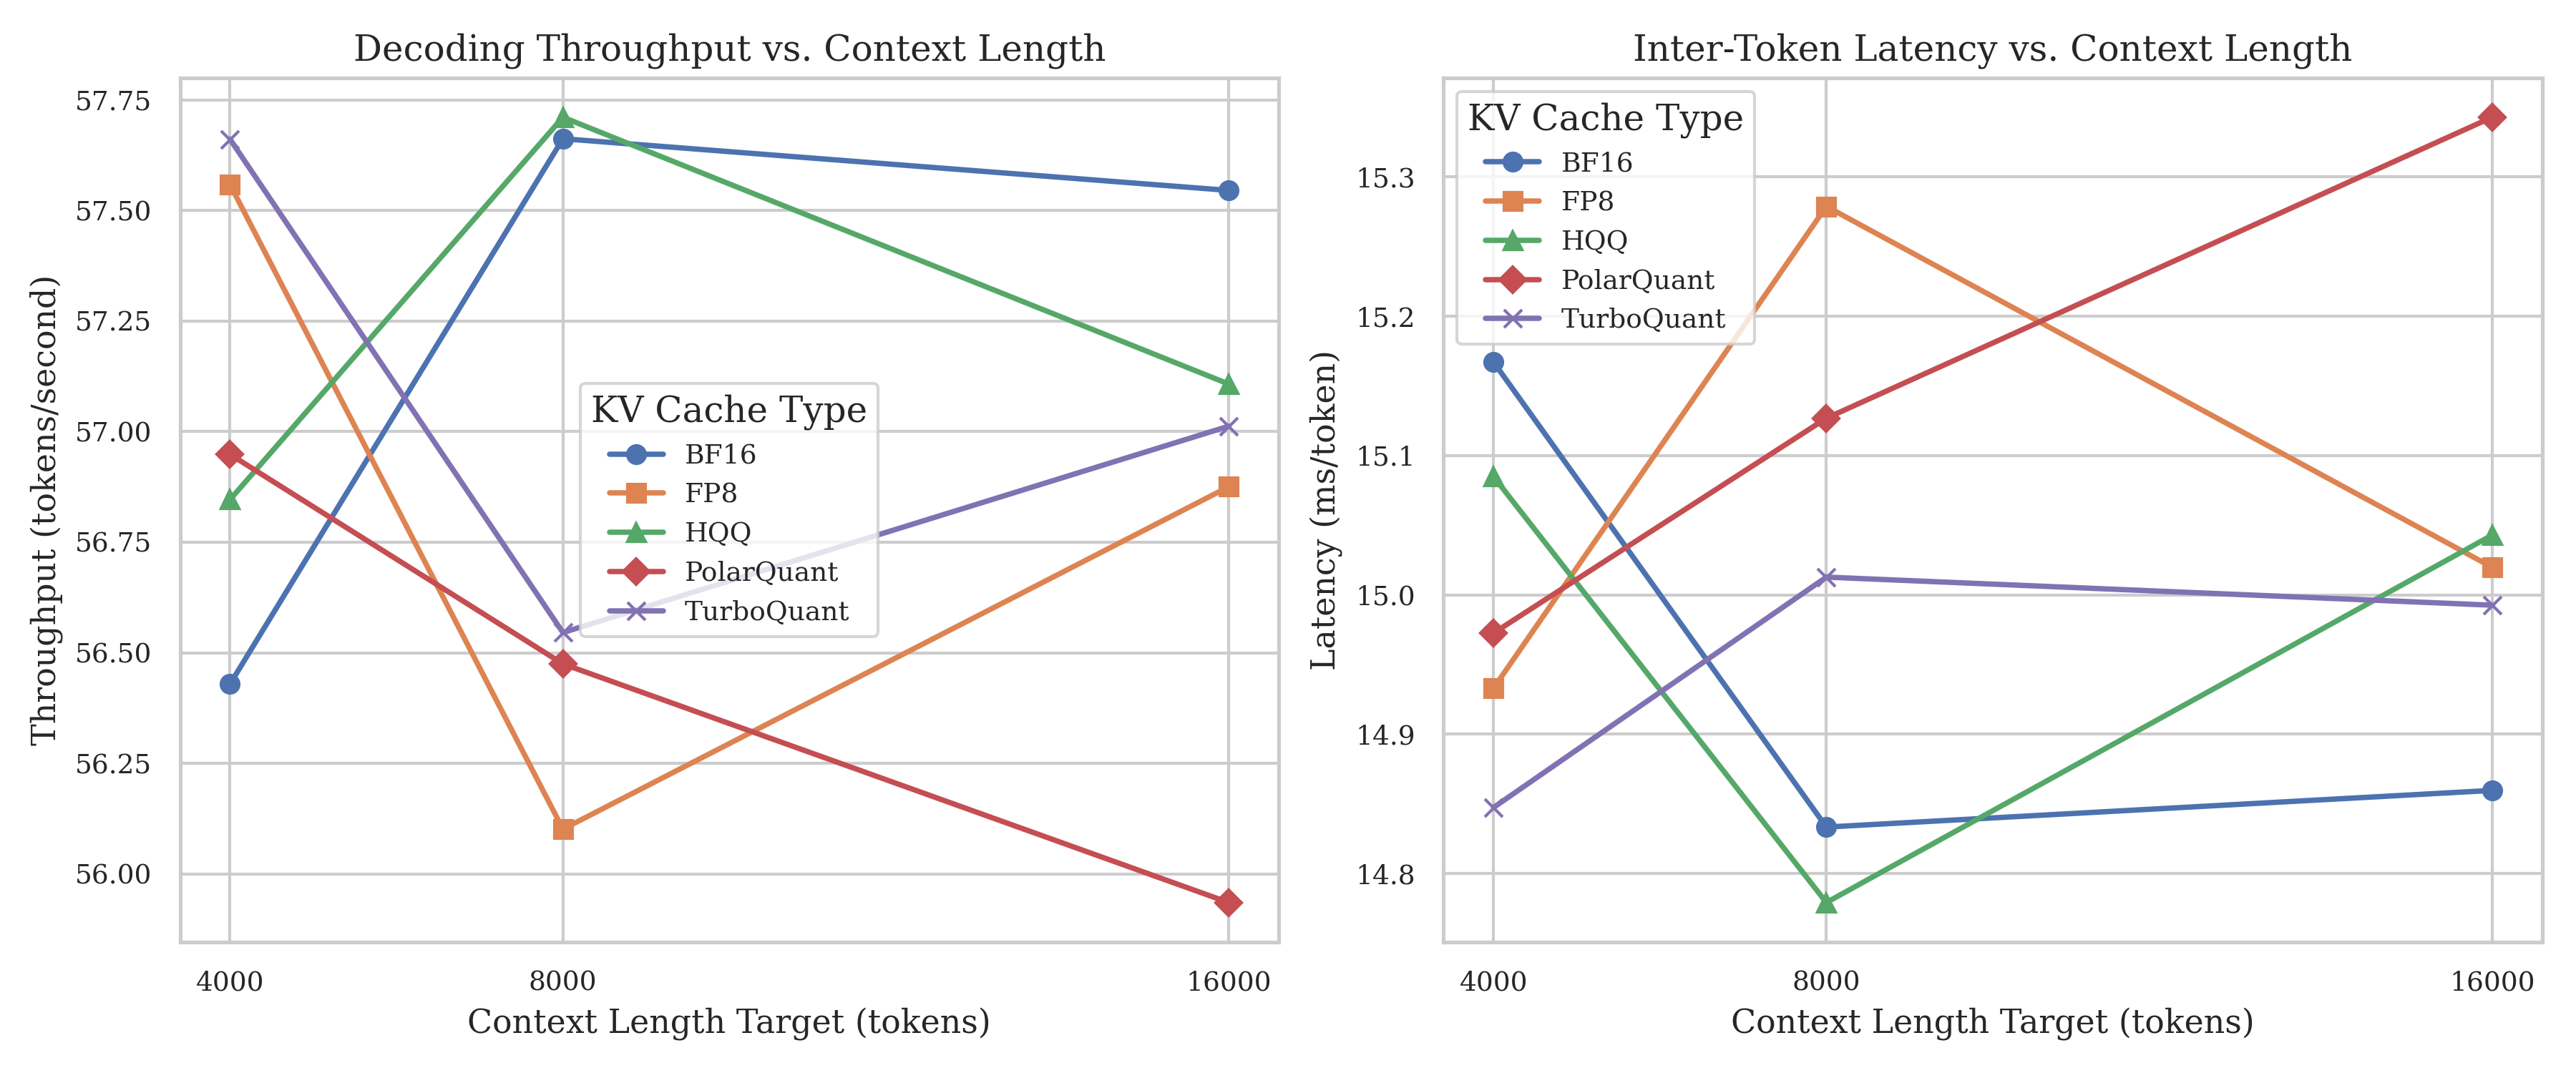
\includegraphics[width=0.45\textwidth]{results/plots/performance_vs_context.png}
\caption{Combined view: decoding throughput (left) and inter-token
latency (right) for all five KV Cache methods across 4k, 8k, and 16k tokens.}
\label{fig:perf_ctx}
\end{figure}

\subsection{Discussion}

\noindent\textbf{Answer to RQ1:}
TurboQuant reduces peak VRAM by up to 0.75\% relative to FP16
(Qwen3-8B at 4k context, $\approx530$~MB), while incurring a
$1.2$--$1.8\times$ latency overhead.
VRAM savings are model-dependent: Qwen3-8B shows consistent reduction
across all context lengths, whereas Qwen2.5-7B-Instruct and Mistral-7B
exhibit only marginal VRAM differences ($<40$~MB) relative to FP16,
indicating that TurboQuant's QJL projection interacts differently
depending on the model's attention architecture.

\noindent\textbf{Answer to RQ2:}
Perplexity degradation under TurboQuant is negligible
($\Delta$PPL~$\approx$~0.03 for Qwen3-8B; overall avg PPL~$\approx1.41$
vs.~FP16 avg~$\approx1.41$ across all three models), confirming that
QJL error-compensation effectively preserves Vietnamese linguistic quality.
In stark contrast, FP8 and PolarQuant cause significant PPL degradation
specifically on Qwen2.5-7B-Instruct: FP8 averages PPL~$\approx4.19$ and
PolarQuant~$\approx3.37$ across the three context lengths, with automated
quality flags (repetition, gibberish) triggered at 8k and 16k context.
HQQ produces the most severe degradation on this model
(avg PPL~$>11$ at 8k--16k), whereas on Qwen3-8B and Mistral-7B its PPL
remains within~$\pm0.1$ of the FP16 baseline.
These findings reveal that Qwen2.5-7B-Instruct is substantially more
sensitive to KV Cache quantization artifacts than the other two models
evaluated---a critical consideration for production deployment.

\noindent\textbf{Answer to RQ3:}
As context length scales from 4k to 16k, all methods experience
near-linear VRAM growth and superlinear latency increase.
The performance gap between FP16 and TurboQuant narrows at 16k context,
suggesting diminishing returns from KV Cache compression at very long contexts.

\noindent\textbf{Answer to RQ4:}
TurboQuant provides the most stable Pareto-optimal boundary:
it is Pareto-dominant over all other methods in the
(Peak VRAM, Perplexity) space.
FP8 is recommended as a drop-in alternative when latency is paramount,
given its near-zero overhead over FP16.
HQQ is not recommended for production deployments above 8k context
due to severe latency degradation.


%========================
\section{Conclusion}
\label{sec:conclusion}
%========================

This paper presented a systematic empirical benchmark of five KV
Cache compression methods---FP16, FP8, HQQ, PolarQuant, and TurboQuant---on
Vietnamese multilingual LLMs across context lengths of 4k, 8k, and 16k tokens.

Our findings demonstrate that \textbf{TurboQuant} achieves the best
Pareto trade-off between peak VRAM reduction and output quality preservation
for Vietnamese text, making it the most suitable choice for
memory-constrained production deployments.
\textbf{PolarQuant} and \textbf{FP8} are strong alternatives when
latency is the primary concern, operating at near-baseline speed
with modest memory savings.
\textbf{HQQ} is not recommended for long-context ($>$8k tokens)
Vietnamese inference due to unacceptable latency overhead.

Future work will extend this benchmark to 32k context lengths,
include additional Vietnamese-specific evaluation tasks (NER, summarization),
and investigate adaptive compression strategies that dynamically
select KV Cache precision based on layer depth and attention entropy.

\medskip
\noindent\textbf{Acknowledgment.}
This research was conducted as the final group project for the course
\emph{Big Data Applications: Machine Learning at Scale (DBML434077)}
at Ho Chi Minh City University of Technology and Engineering (HCM-UTE),
under the supervision of Dr.~Le Ngoc Hieu.
The authors thank the open-source communities behind vLLM, NVIDIA NeMo Curator,
VTSNLP, and VMLU for providing the infrastructure and data that made
this work possible.


%========================
% BIBLIOGRAPHY
%========================

\bibliographystyle{IEEEtran}
\bibliography{references}



\end{document}
